\chapter{Эксперимент}
\label{cha:research}

\section{Ход работы}

В среду были добавлены искусственные баги, которые проявляются при первом посещении агентом областей \(x \in (-0,9; -0.8)\) и \(x \in (0,75; 0.8)\). Эти участки обозначены красным цветом на рис.~\ref{fig:bugLocations}. Интервалы были выбраны так, чтобы они находились вне стандартной траектории посадки и требовали отклонения от курса.

\begin{figure}
	\centering
	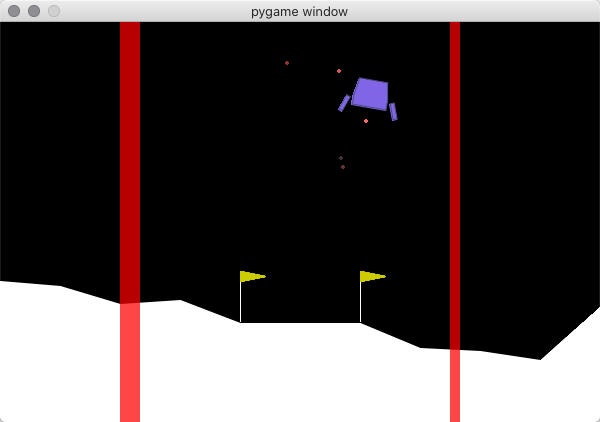
\includegraphics[width=0.75\textwidth]{figures/bug locations}
	\caption{Области проявления багов.}
	\label{fig:bugLocations}
\end{figure}

За первое посещение каждой из областей лендер получает награду в \(+250\) единиц. После этого в этом эпизоде баг не проявляется, и для максимизации награды агенту остается совершить посадку. Первичные тесты показали, что награда при попадании в заданные интервалы плохо мотивировала модель на отклонение от оптимального курса посадки (даже при её увеличении), поэтому было решено добавить штраф в \(-50\) единиц, если агент завершает эпизод, не найдя ни одного бага. Более высокие штрафы здесь не подошли, т.~к. они мотивируют агента вовсе избегать посадки на площадку.

Гиперпараметры модели были подобраны эмпирически с целью достижения исходной моделью среднего счета за последние 100 эпизодов в >200 единиц. Тогда создатели считают среду <<разрешенной>> \cite{lunarlanderv2}.

\section{Результаты эксперимента}

\begin{table}[ht]
	\centering
	\caption{Число эпизодов (из 100), в которых модели нашли хотя бы один баг.}
	\begin{tabular}{ l r r r }
		\hline
		№ & \makecell[r]{Итоговая\\D3QN} & \makecell[r]{Исходная\\D3QN} & Случайный агент \\
		\hline
		1 & 49 & 0 & 22\\
		2 & 38 & 0 & 23\\
		3 & 37 & 0 & 21\\
		4 & 42 & 0 & 20\\
		5 & 42 & 0 & 24\\
		6 & 46 & 0 & 27\\
		7 & 49 & 0 & 26\\
		8 & 39 & 0 & 14\\
		9 & 54 & 0 & 14\\
		10 & 39 & 0 & 19\\
		\hline
		\textit{среднее} & 43,5 & 0 & 21 \\
		\textit{медиана} & 42 & 0 & 21,5 \\
		\textit{ср.~кв.~отклонение} & 5,72 & 0 & 4,447 \\
		\hline
	\end{tabular}
	\label{tab:results}
\end{table}

Полученная модель D3QN тренировалась в течение 250 эпизодов. После этого, натренированный агент дополнительно проходил ещё 100 последовательных эпизодов, записывая число найденных багов на каждом. 

Из-за того, что поверхность Луны и сила, приложенная к центру масс модуля различаются от эпизода к эпизоду, тесты были проведены 10 раз для получения усредненных значений.

Производительность модели сравнивается с исходной D3QN, которая не получала награду за нахождение багов на этапе тренировки, а также с агентом, который на каждом шаге выбирает случайное действие. Результаты эксперимента приведены в табл.~\ref{tab:results}. 

Результаты показывают, что исходная модель D3QN вовсе не справляется с задачей поиска ошибок. Агент модифицированной D3QN смог показать лучший результат среди всех трех: это говорит о том, что награда, полученная за нахождение багов побуждает модель их искать, даже если это негативно влияет на посадку модуля.

%%% Local Variables:
%%% mode: latex
%%% TeX-master: "rpz"
%%% End:
